\def\dlt{0.4}
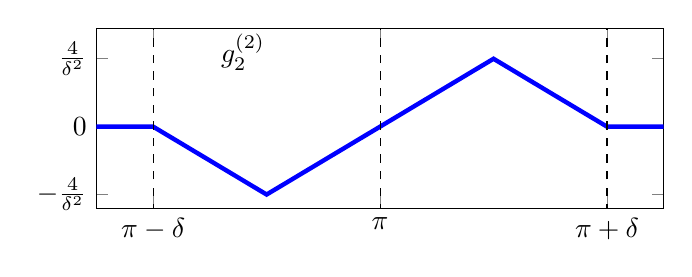
\begin{tikzpicture}
\begin{axis}[
    width=250pt,height=110pt,
    xmin=pi-0.5,xmax=pi+0.5,
    ymin=-1.2,ymax=1.45,
    samples=50,
    xtick={pi-\dlt, pi, pi+\dlt},
    xticklabels={$\pi - \delta$, $\pi$, $\pi + \delta$},
    ytick={-1, 0, 1},
    yticklabels={$-\frac{4}{\delta^2}$, $0$, $\frac{4}{\delta^2}$},
    grid style={line width=.1pt, draw=gray!10}]

    \addplot[blue, ultra thick] coordinates {
        (0, 0) (pi-\dlt, 0) (pi-\dlt/2, -1) (pi+\dlt/2, 1) (pi+\dlt, 0) (4,0)
    };

    \draw [dashed] (axis cs:{pi-\dlt},-2) -- (axis cs:{pi-\dlt},2);
    \draw [dashed] (axis cs:{pi},-2) -- (axis cs:{pi},2);
    \draw [dashed] (axis cs:{pi+\dlt},-2) -- (axis cs:{pi+\dlt},2);
    
    \node at (axis cs:2.9,1.1) {$g^{(2)}_2$};
\end{axis}
\end{tikzpicture}
\undef\dlt